\chapter{Teaching as a Performance Art}\label{s:performance}

As Chapter~\ref{s:pck} explained, every teacher needs content knowledge,
general pedagogical knowledge, and pedagogical content knowledge in
order to be effective. We can elaborate this framework by adding
technology to the mix \cite{Koeh2013}, but that doesn't change the
key point: it isn't enough to know the subject, or how to teach---you have
to know how to teach that particular subject \cite{Maye2004}.

This chapter therefore focuses on one key aspect of teaching: giving a
lecture or a live demonstration in front of a class. It isn't the only
way to teach, but it is probably the most common, and the techniques
that will make you better at doing it can be applied elsewhere as well.

\begin{aside}{Teaching Tips}

The \hreffoot{http://csteachingtips.org/}{CS Teaching Tips} site is collecting PCK for
teaching programming, and I hope that one day we will have catalogs
like \cite{Ojos2015}, teacher training materials like
\cite{Hazz2014,Guzd2015a,Sent2018}, or more
personal collections like \cite{Gelm2002} to help us all do it
better.

\end{aside}

\section{Lesson Study}\label{s:performance-jugyokenkyu}

From politicians to researchers and teachers themselves, educational
reformers have designed systems to find and promote people who can teach
well and eliminate those who cannot. But the assumption that some people
are born teachers is wrong; instead, like any other performance art, the
keys to better teaching are practice and collaboration. As
\cite{Gree2014} explains, the Japanese approach to this is called
\gref{g:jugyokenkyu}{jugyokenkyu}, which means ``lesson study'':

\begin{quote}

\emph{Jugyokenkyu} is a bucket of practices that Japanese teachers use to
hone their craft, from observing each other at work to discussing the
lesson afterward to studying curriculum materials with colleagues. The
practice is so pervasive in Japanese schools that it
is{\ldots}effectively invisible.

In order to graduate, {[}Japanese{]} education majors not only had to
watch their assigned master teacher work, they had to effectively
replace him, installing themselves in his classroom first as
observers and then, by the third week, as a wobbly{\ldots}approximation
of the teacher himself. It worked like a kind of teaching
relay. Each trainee took a subject, planning five days' worth of
lessons{\ldots} {[}and then{]} each took a day. To pass the baton, you had to
teach a day's lesson in every single subject: the one you planned
and the four you did not{\ldots} and you had to do it right under your
master teacher's nose. Afterward, everyone---the teacher, the
college students, and sometimes even another outside
observer---would sit around a formal table to talk about what they
saw.

\end{quote}

Putting work under a microscope in order to improve it is commonplace
in sports and music. A professional musician, for example, will
dissect half a dozen different recordings of ``Body and Soul'' or
``Smells Like Teen Spirit'' before performing it. She would also expect
to get feedback from fellow musicians during practice and after
performances. Many other professions work this way as well: for
example, the Japanese drew inspiration from \hreffoot{https://en.wikipedia.org/wiki/W.\_Edwards\_Deming}{Deming's ideas on
continuous improvement in manufacturing}.

But continuous feedback isn't part of teaching culture in most
English-speaking countries. There, what happens in the classroom stays
in the classroom: teachers don't watch each other's lessons on a
regular basis, so they can't borrow each other's good ideas. The
result is that \emph{every teacher has to invent teaching on their
own}. They may get lesson plans and assignments from colleagues, the
school board or a textbook publisher, or go through a few MOOCs on the
Internet, but each teacher has to figure out for herself how to
combine that content with the theory she learned in education school
to deliver an actual lesson in an actual classroom for actual
students.

Writing up new techniques and giving \gref{g:demonstration-lesson}{demonstration
lessons}, in which one person teaches actual
students while other teachers observe, seem like a way to solve
this. However, \cite{Finc2007,Finc2012} found that they
are usually ineffective: of the 99 change stories analyzed, teachers
only searched actively for new practices or materials in three cases,
and only consulted published material in eight cases. Most changes
occurred locally, without input from outside sources, or involved only
personal interaction with other educators.

\cite{Bark2015} found something similar:

\begin{quote}

Adoption is not a ``rational action,'' however, but an iterative series
of decisions made in a social context, relying on normative
traditions, social cueing, and emotional or intuitive
processes{\ldots} Faculty are not likely to use educational
research findings as the basis for adoption decisions{\ldots}
Positive student feedback is taken as strong evidence by faculty that
they should continue a practice.

\end{quote}

This phenomenon is sometimes called \gref{g:lateral-knowledge-transfer}{lateral knowledge
transfer}: someone sets out to teach X,
but while watching them, their audience actually learns Y as well (or
instead). For example, a teacher might intend to show learners how to
search for email addresses in a text file, but what her audience might
take away is some new keyboard shortcuts in the editor. What
\emph{jugyokenkyu} does is maximize the opportunity for this to happen
between teachers.

\section{Giving and Getting Feedback on Teaching}\label{s:performance-feedback}

Observing someone helps you; giving them feedback helps them. But as the
cartoon in Figure~\ref{f:performance-feedback-feelings} suggests, it can
be hard to receive feedback, especially when it's negative.

\begin{figure}
\centering
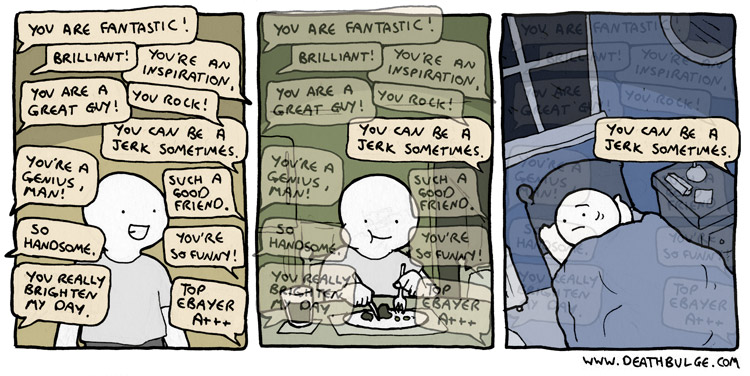
\includegraphics{../../figures/deathbulge-jerk.jpg}
\caption{Feedback Feelings (copyright © Deathbulge 2013)}
\label{f:performance-feedback-feelings}
\end{figure}

Feedback is easier to give and receive when both parties share ground
rules and expectations. This is especially important when they have
different backgrounds or cultural expectations about what's appropriate
to say and what isn't. You can get better feedback on your work by using
these techniques:

\begin{description}
\item[Initiate feedback.]
It's better to ask for feedback than to receive it unwillingly.
\item[Choose your own questions,]
i.e., ask for specific feedback. It's a lot harder for someone to
answer, ``What do you think?'' than to answer either, ``What is one
thing I could have done as a teacher to make this lesson more
effective?'' or ``If you could pick one thing from the lesson to go
over again, what would it be?''

Directing feedback like this is also more helpful to you. It's
always better to try to fix one thing at once than to change
everything and hope it's for the better. Directing feedback at
something you have chosen to work on helps you stay focused, which
in turn increases the odds that you'll see progress.
\item[Use a feedback translator.]
Have someone else read over all the feedback and give you a summary.
It can be easier to hear ``It sounds like most people are following,
so you could speed up'' than to read several notes all saying, ``this
is too slow'' or ``this is boring''.
\item[Be kind to yourself.]
Many of us are very critical of ourselves, so it's always helpful to
jot down what we thought of ourselves \emph{before} getting feedback from
others. That allows us to compare what we think of our performance
with what others think, which in turn allows us to scale the former
more accurately. For example, it's very common for people to think
that they're saying ``um'' and ``err'' all the time, when their audience
doesn't notice it. Getting that feedback once allows teachers to
adjust their assessment of themselves the next time they feel that
way.
\end{description}

You can give feedback to others more effectively as well:

\begin{description}
\item[Balance positive and negative feedback.]
A common method is a ``compliment sandwich'' made up of one positive,
one negative, and a second positive observation (though this can get
tiresome after a while).
\item[Organize your feedback using a rubric.]
Most people are more comfortable giving and receiving feedback when
they feel that they understand the social rules governing what they
are allowed to say and how they are allowed to say it. A facilitator
can then transcribe items into a shared document (or onto a
whiteboard) during discussion.
\end{description}

The simplest rubric for feedback on teaching is a 2x2 grid whose
vertical axis is labelled ``what went well'' and ``what can be improved'',
and whose horizontal axis is labelled ``content'' (what was said) and
``presentation'' (how it was said). Observers write their comments on
sticky notes as they watch the demonstration, then post those in the
quadrants of a grid drawn on a whiteboard
(Figure~\ref{f:performance-rubric}).

\begin{figure}
\centering
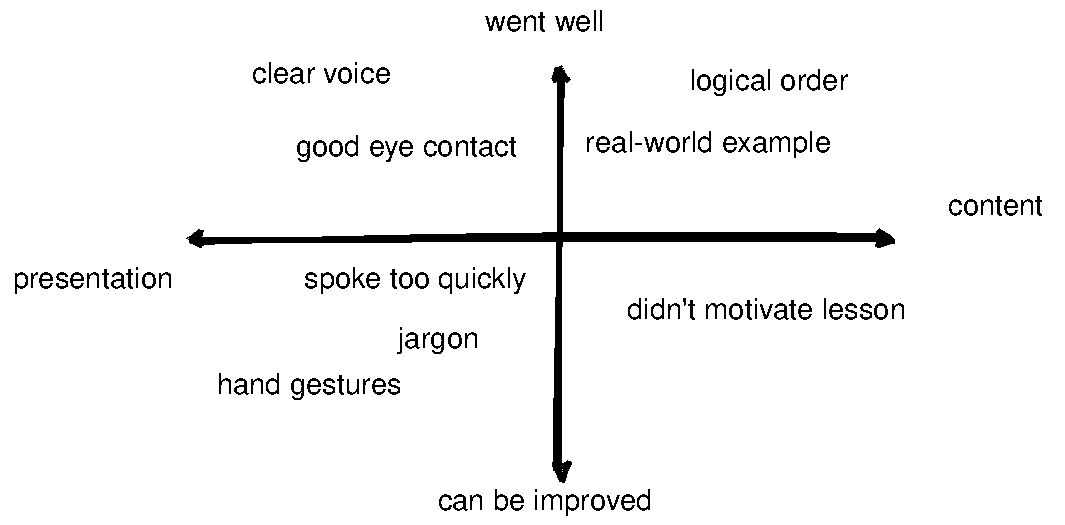
\includegraphics{../../figures/2x2-rubric.pdf}
\caption{Teaching Rubric}
\label{f:performance-rubric}
\end{figure}

A more sophisticated rubric developed for assessing 5--10 minute videos
of programming instruction is given in Section~\ref{s:checklists-teacheval}. A
rubric this detailed is best presented as a checklist with items more or
less in the order that they'll be used (e.g., questions about the
introduction come before questions about the conclusion).

\begin{aside}{Question Budgets}

Rubrics like the one in Section~\ref{s:checklists-teacheval} have a tendency to
grow over time as people think of things they'd like to add. A good
way to keep them manageable is to insist that the total length stay
constant, i.e., that if someone wants to add a question, they have to
identify one that's less important and can be removed.

\end{aside}

If you are interested in giving and getting feedback, \cite{Gorm2014}
has good advice that you can use to make peer-to-peer feedback a routine
part of your teaching, while \cite{Gawa2011} looks at the value of
having a coach. However feedback is collected, remember that it is meant
to be formative: its goal is to help people figure out what they are
doing well and what they still need to work on. Please also remember
that these guidelines are for peer-to-peer feedback on your lesson
delivery; gathering feedback from your learners should be as close to
continuous as you can make it, and you should prompt for questions and
reflections as well as positives and negatives.

\begin{aside}{Studio Classes}

Architecture schools often include studio classes, in which students
solve small design problems and get feedback from their peers right
then and there. These classes are most effective when the teacher
critiques both the designs and the peer critiques, so that
participants learn not only how to make buildings, but how to give and
get feedback \cite{Scho1984}. Master classes in music serve a
similar purpose.

\end{aside}

\section{How to Practice Performance}\label{s:performance-practice}

The best way to improve your in-person lesson delivery is to watch
yourself do it. This method is borrowed from Warren Code at the
University of British Columbia.

\begin{enumerate}
\item
  Work in groups of three.
\item
  Each person rotates through the roles of teacher, audience, and
  videographer. The teacher has two minutes to explain one key idea
  from their teaching or other work as if they were talking to a class
  of high school students. The person pretending to be the audience is
  there to be attentive, while the videographer records the session
  using a cellphone or other handheld device.
\item
  After everyone has finished teaching, the whole group watches the
  videos together. Everyone gives feedback on all three videos, i.e.,
  people give feedback on themselves as well as on others.
\item
  After the videos have been discussed, they are deleted. (Many people
  are increasingly uncomfortable with the prospect of images of
  themselves appearing online.)
\item
  Finally, return to the main group and add the feedback to a shared
  2x2 grid that separates positive from negative and content from
  presentation.
\end{enumerate}

In order for this exercise to work well:

\begin{itemize}
\item
  Record all three videos and then watch all three. If the cycle is
  teach-review-teach-review, the last person to teach runs out of
  time. Doing all the reviewing after all the teaching also helps put
  a bit of distance between the teaching and the reviewing, which
  makes the exercise slightly less excruciating.
\item
  Let people know at the start of the class that they will be asked to
  teach something so that they have time to choose a topic. (Telling
  them this in advance can be counter-productive, since some people
  will fret over how much they should prepare.)
\item
  Groups must be physically separated to reduce audio cross-talk
  between their recordings. In practice, this means 2--3 groups in a
  normal-sized classroom, with the rest using nearby breakout spaces,
  coffee lounges, offices, or (on one occasion) a janitor's storage
  closet.
\item
  People must give feedback on themselves, as well as giving feedback
  on each other, so that they can calibrate their impressions of their
  own teaching according to the impressions of other people. (Most
  people are harder on themselves than others are, and it's important
  for them to realize this.)
\end{itemize}

The announcement of this exercise is often greeted with groans and
apprehension, since few people enjoy seeing or hearing themselves.
However, those same people consistently rate it as one of the most
valuable parts of workshops based on these notes. It's also good
preparation for co-teaching (Section~\ref{s:classroom-together}):
teachers find it a lot easier to give each other informal feedback if
they have had some practice doing so and have a shared rubric to set
expectations.

\begin{aside}{Tells}

Everyone has nervous habits. For example, many of us talk more rapidly
and in a higher-pitched voice than usual, while others play with their
hair or crack their knuckles. Gamblers call nervous habits like this
``tells''. While these are often not as noticeable as you would think,
it's good to know whether you pace, fiddle with your hair, look at
your shoes, or rattle the change in your pocket when you don't know
the answer to a question.

You can't get rid of tells completely, and trying to do so can make
you obsess about them. A better strategy is to try to displace them,
e.g., to train yourself to scrunch your toes inside your shoes instead
of cracking your knuckles.

\end{aside}

\section{Live Coding}\label{s:performance-live}

\begin{quote}

  Teaching is theater, not cinema. \\
  --- Neal Davis

\end{quote}

One technique that completely changed the way I teach programming is
\gref{g:live-coding}{live coding}. Instead of using slides,
teachers actually write code in front of their class as their learners
follow along. It's more effective than slides for many reasons:

\begin{itemize}
\item
  Watching a program being written is more compelling than watching
  someone page through slides that present bits and pieces of the same
  code.
\item
  It enables teachers to be more responsive to ``what if?'' questions.
  Where a slide deck is like a railway track, live coding allows
  teachers to go off road and follow their learners' interests.
\item
  It facilitates lateral knowledge transfer: people learn more than we
  realized we were teaching by watching \emph{how} teachers do things.
\item
  It slows the teacher down: if she has to type in the program as she
  goes along, she can only go twice as fast as her learners, rather
  than ten-fold faster as she could with slides.
\item
  It helps to keep the load on short-term memory down because it makes
  the teacher more aware of how much they are throwing at their
  learners. (This isn't true of slides or of copy-and-paste.)
\item
  Learners get to see teachers' mistakes \emph{and how to diagnose and
  correct them}. Novices are going to spend most of their time doing
  this, but it's left out of most textbooks.
\item
  Watching teachers make mistakes shows learners that it's all right
  to make mistakes of their own. Most people model the behavior of
  their teachers: if the teacher isn't embarrassed about making and
  talking about mistakes, learners will be more comfortable doing so
  too.
\end{itemize}

Teachers need a bit of practice to get comfortable with thinking aloud
as they code in front of an audience, but most report that it is then no
more difficult than talking around a deck of slides, and research seems
to back up its effectiveness \cite{Rubi2013,Haar2017}. The sections
below offer tips on how to make your live coding better.

\subsection*{Embrace Your Mistakes}

\begin{quote}

  The typos are the pedagogy. \\
  --- Emily Jane McTavish

\end{quote}

The most important rule of live coding is to embrace your mistakes. No
matter how well you prepare, you will make some; when you do, think
through them with your audience. While data is hard to come by,
professional programmers spend anywhere from 25\% to 60\% of their time
debugging; novices spend much more (Section~\ref{s:pck-debug}), but most
textbooks and tutorials spend little time diagnosing and correct
problems. If you talk aloud while you figure out what you mistyped or
where you took the wrong path, and explain how you've corrected
yourself, you will give your learners a toolbox they can use when they
make their own mistakes.

This is at odds with advice like that in \cite{Kran2015}, which
says, ``{\ldots}you should have your material \emph{absolutely mastered} before
you enter the classroom. If{\ldots}you have a proof or example that is not
quite right{\ldots}and stand in front of the group trying to fix it, then
you will lose all but the diehards quickly.'' In contrast, the feedback
we've had in \hreffoot{http://software-carpentry.org}{Software Carpentry} workshops and other settings is
that watching the teacher make mistakes actually motivates most
students, since it gives them permission to be less than perfect as
well.

\begin{aside}{Deliberate Fumbles}

If you've given a lesson several times, you're unlikely to make
anything other than basic typing mistakes (which can still be
informative). You can try to remember past mistakes and make them
deliberately, but that often feels forced (unless the mistake and
how to correct it is the primary purpose of the lesson). A better
approach is sometimes called \gref{g:twitch-coding}{twitch coding}: ask
learners one by one to tell you what to type next. This is pretty
much guaranteed to get you into the weeds.

\end{aside}

\subsection*{Ask For Predictions}

One way to keep students engaged while you are live coding is to ask
them to make predictions, e.g., to say, ``What is going to happen when I
run this code?'' You can then either show them, or write down the first
few suggestions they make, have the whole class vote on which they think
is most likely, and then run the code. As well as keeping their
attention on task, this gives them practice at reasoning about code's
behavior, which is a useful skill in its own right.

\subsection*{Take It Slow}

For every command you type, every word of code you write, every menu
item or website button you click, say out loud what you are doing while
you do it, then point to the command and its output on the screen and go
through it a second time. This not only slows you down, it allows
learners who are following along to copy what you do, or to catch up,
even when they are looking at their screen while doing it. Whatever you
do, \emph{don't} copy and paste code: doing this practically guarantees that
you'll race ahead of your learners. And if you use tab completion, say
it out loud the first few times so that your learners understand what
you're doing: ``Let's use turtle dot `r' `i' and tab to get `right'.''

If the output of your command or code makes what you just typed
disappear from view, scroll back up so learners can see it again. If
that's not practical, execute the same command a second time, or copy
and paste the last command(s) into the workshop's shared notes.

\subsection*{Be Seen and Heard}

If you are physically able to stand up for a couple of hours, do it
while you are teaching. When you sit down, you are hiding yourself
behind others for those sitting in the back rows. Make sure to notify
the workshop organizers of your wish to stand up and ask them to arrange
a high table, standing desk, or lectern.

Regardless of whether you are standing or sitting, make sure to move
around as much as reasonable. You can for example go to the screen to
point something out, or draw something on the white/blackboard (see
below). Moving around makes the teaching more lively, less monotonous.
It draws the learners' attention away from their screens, to you, which
helps get the point you are making across.

Even though you may have a good voice and know how to use it well, it
may be a good idea to use a microphone, especially if the workshop room
is equipped with one. Your voice will be less tired, and you increase
the chance of people with hearing difficulties being able to follow the
workshop.

\subsection*{Mirror Your Learner's Environment}

You may have customized your environment with a fancy Unix shell prompt,
a custom color scheme for your development environment, or a plethora of
keyboard shortcuts. Your learners won't have any of this, so try to
create an environment that mirrors what they \emph{do} have. Some teachers
create a separate bare-bones user (login) account on their laptop, or a
separate teaching-only account if they're using an online service like
Scratch or GitHub.

\subsection*{Use the Screen Wisely}

You will need to enlarge your font considerably in order for people to
read it from the back of the room, which means you can put much less on
the screen than you're used to. You will often be reduced to 60--70
columns and 20--30 rows, which basically means that you're using a 21st
Century supercomputer to emulate an early-1980s VT100 terminal.

To cope with this, maximize your window, and then ask everyone to give
you a thumbs-up or thumbs-down on its readability. Use a black font on a
lightly-tinted background rather than a light font on a dark
background---the light tint will glare less than a pure white
background.

Pay attention to the room lighting as well: it should not be fully dark,
and there should be no lights directly on or above the presenter's
screen. If needed, reposition the tables so all learners can see the
screen.

When the bottom of the projector screen is at the same height, or below,
the heads of the learners, people in the back won't be able to see the
lower parts. Raise the bottom of your window(s) to compensate, but be
aware that this gives you even less space for your typing.

If you can get a second projector and screen, use it: the extra real
estate will allow you to display your code on one side and its output or
behavior on the other. The second screen may require its own PC or
laptop, so you may need to ask a helper to control it.

If you teach using a console window, such as a Unix shell, it's
important to tell people when you run an in-console text editor and when
you return to the console prompt. Most novices have never seen a window
take on multiple personalities in this way, and can quickly become
confused (particularly if the window is hosting an interactive
interpreter prompt for Python or some other language as well as running
shell commands and hosting an editor).

\begin{aside}{Accessibility Aids Help Everyone}

Tools like \hreffoot{https://boinx.com/mousepose/overview/}{Mousepos\'{e}} (for Mac) and
\hreffoot{http://www.pointerfocus.com/}{PointerFocus} (for Windows) will highlight the
position of your mouse cursor on the screen, and screen recording
software tools like \hreffoot{https://www.techsmith.com/video-editor.html}{Camtasia} will echo invisible keys
like tab and Control-J as you type them. These take a bit of
practice to get used to, but are extremely helpful as you start
teaching more advanced tools.

\end{aside}

\subsection*{Double Devices}

Some people now use two devices when teaching: a laptop plugged into the
projector for learners to see, and a tablet beside it so that they can
view their own notes and the shared notes that the learners are taking
together (Section~\ref{s:classroom-notetaking}). This is more reliable
than displaying one virtual desktop while flipping back and forth to
another. Of course, printouts of the lesson material are still the most
reliable backup technology{\ldots}

\subsection*{Use Diagrams}

Diagrams are almost always a good idea. Creating them in advance to
bring up on screen is a common practice---I often have a slide deck full
of diagrams in the background when I'm doing live coding---but don't
underestimate the value of sketching on the whiteboard as you go through
your lesson. This allows you to build diagrams step by step, which helps
with retention (Section~\ref{s:load-split-attention}) and allows you to
improvise.

\subsection*{Avoid Distractions}

Turn off any notifications you may use on your laptop, such as those
from social media, email, etc. Seeing notifications flash by on the
screen distracts you as well as the learners, and it can be awkward when
a message pops up you'd rather not have others see. If you are teaching
frequently, you might want to create a second account on your computer
that doesn't have email or other tools set up at all.

\subsection*{Improvise After You Know the Material}

The first time you teach a new lesson, stick fairly closely to the
lesson plan you've drawn up or borrowed. It may be tempting to deviate
from the material because you would like to show a neat trick or
demonstrate some alternative way of doing something. Resist: there is a
fair chance you'll run into something unexpected that you then have to
explain.

Once you are more familiar with the material, though, you can and should
start improvising based on the backgrounds of your learners, their
questions in class, and what you find most interesting about the lesson.
This is like playing a new song: the first few times, you stick to the
sheet music, but after you're comfortable with it, you can start to put
your own stamp on it.

If you really want to use something outside of the material, run through
it beforehand as you plan to in class \emph{using the same computer that
you'll be teaching on}. Installing several hundred megabytes of
software updates over high school WiFi in front of increasingly bored
16-year-olds isn't something you want to do twice.

\begin{aside}{Direct Instruction}

\gref{g:direct-instruction}{Direct Instruction} is a teaching
method centered around meticulous curriculum design delivered through
a prescribed script---i.e., it's more like an actor reciting lines than
it is like the improvisatory approach we recommend. \cite{Stoc2018}
surveys studies and finds statistically significant positive effect,
even though DI sometimes gets knocked for being mechanical. We still
prefer improvisation because DI requires a far greater up-front
investment than most free-range learning groups can afford.

\end{aside}

\subsection*{Face the Screen---Occasionally}

It's OK to face the screen occasionally, particularly when you are
walking through a section of code statement by statement or drawing a
diagram, but you shouldn't do this for more than a few seconds at a
time. Looking at the screen for a few seconds can help lower your
anxiety levels, since it gives you a brief break from being looked at.

A good rule of thumb is to treat the screen as one of your learners: if
it would be uncomfortable to stare at someone for as long as you are
spending looking at the screen, it's time to turn around and face your
audience.

\subsection*{Drawbacks}

Live coding does have some drawbacks, but with practice, these can be
avoided or worked around. A common one is going too slowly, either
because you are not a good typist or because you are spending too much
time looking at notes trying to figure out what to type next. The fix
for the first is a bit of typing practice; the fix for the second is to
break the lesson into very short pieces, so that you only ever have to
remember one small step to take next.

A deeper exercise is that typing in library import statements, class
headers, and other boilerplate code increases the extraneous cognitive
load on your learners (Chapter~\ref{s:load}). If you spend a lot of time
doing this, it may be all that learners take away, so give yourself and
your learners skeleton code to start with
(Section~\ref{s:classroom-blank}).

\section{Exercises}\label{s:performance-exercises}

\subsection*{Give Feedback on Bad Teaching (whole class/20)}

\begin{enumerate}
\item
  Watch \hreffoot{https://www.youtube.com/watch?v=-ApVt04rB4U}{this video of bad teaching} as a group
  and give feedback on it. Organize feedback along two axes: positive
  vs. negative and content vs. presentation.
\item
  Have each person in the class add one point to a 2x2 grid on a
  whiteboard (or in the shared notes) without duplicating any points
  that are already up there.
\end{enumerate}

What did other people see that you missed? What did they think that you
strongly agree or disagree with?

\subsection*{Practice Giving Feedback (small groups/45)}

Use the process described above to practice teaching in groups of
three. When your group is done, the teacher will add one point of
feedback from each participant to a 2x2 grid on the whiteboard or in
the shared notes, without accepting duplicates. Participants should
not say whether the point they offer was made by them, about them, or
neither: the goal at this stage is primarily for people to become
comfortable with giving and receiving feedback, and to establish a
consensus about what sorts of things to look for.

\subsection*{The Bad and the Good (whole class/20)}

Watch the videos of \hreffoot{https://youtu.be/bXxBeNkKmJE}{live coding done poorly}
and \hreffoot{https://youtu.be/SkPmwe\_WjeY}{live coding done well} and summarize your
feedback on both using the usual 2x2 grid. These videos assume
learners know what a shell variable is, know how to use the \texttt{head}
command, and are familiar with the contents of the data files being
filtered.

\subsection*{See Then Do (pairs/30)}

Teach 3--4 minutes of a lesson using live coding to a fellow trainee,
then swap and watch while that person live codes for you. Don't bother
trying to record the live coding sessions---we have found that it's
difficult to capture both the person and the screen with a handheld
device---but give feedback the same way you have previously (positive and
negative, content and presentation). Explain in advance to your fellow
trainee what you will be teaching and what the learners you teach it to
are expected to be familiar with.

\begin{itemize}
\item
  What felt different about live coding (versus standing up and
  lecturing)? What was harder/easier?
\item
  Did you make any mistakes? If so, how did you handle them?
\item
  Did you talk and type at the same time, or alternate?
\item
  How often did you point at the screen? How often did you highlight
  with the mouse?
\item
  What will you try to do differently next time?
\end{itemize}

\subsection*{Tells (small groups/15)}

\begin{enumerate}
\item
  Read the description of tells at the end of
  Section~\ref{s:performance-feedback}, then make a note of what you
  think your tells are, but do not share them with other people.
\item
  Teach a short (3--5 minute) lesson.
\item
  Ask your audience how they think you betray nervousness. Is their
  list the same as yours?
\end{enumerate}

\subsection*{Teaching Tips (small groups/15)}

The \hreffoot{http://csteachingtips.org/}{CS Teaching Tips} site has a large number of
practical tips on teaching computing, as well as a collection of
downloadable tip sheets. In small groups, go through the tip sheets on
their home page and classify each tip as ``use all the time'', ``use
occasionally'', ``never use''. Where do your practice and your peers'
practice differ? Are there any tips you strongly disagree with, or
think would be ineffective?
